% STATUS: SUPERSEDED-BY reference/eq17_analysis/derivation/motion_ctrl.tex (part2_conly S2.1-2.5 = this file S1-S5 verbatim; 2026-10-05)
% (was ACTIVE) -- c-only slope law (p = 2): process noise Q55 of the constant c, Q55 = P_fix^2 I[k] (constant variance P^f_55 = P_fix), from F_e, H and the KF.
% Wording (user 10-05): no 'slot', no 'lines', 'information' (not 'evidence'); the code name of this choice is q55_adapt = 'ratio'
%   (0930 Q/R-ratio derivation); the document names it by what it does.
% ======================================================
% Compile: xelatex 1004_q55_ratio_from_kf.tex   (from reference/eq17_analysis/derivation/)
% F_e, H: the slope-law SSOT 0921_estb_v2_slope_c.tex at p = 2 (same as 0928_obs_c_only_v1.tex S1).
% Kalman filter lines: 0929_kf_two_tracks.tex S2 (Meng 2025, Sec. II.F).  I_k: 0930_q55_ratio_design.tex (here I[k]); 0930 P_0 = P_fix here (user 10-04: P_0 = the start value P^f_55[0], P_fix = the equilibrium).
% Code: motion_control_law_formC_b.m, law 'f1p2' (slot 5 = c), q55_adapt = 'ratio':
%   I[k]  -> line 2621  q55a_I = max(0, 1/P_upd(5,5) - 1/P_pred(5,5))      (P_upd = P[k], P_pred = P^f[k])
%   Q55   -> line 2086  qadd = q55a_P0^2 * q55a_I                           (q55_adapt_P0 = sqrt(P_fix); P_0 = opts.sig^2 in run_plaw_walls)
%   F_e row 5 = [0 0 0 0 1] -> local_build_F_e_formC (row 5 = identity)
% Row-5 identities checked numerically against a full 5x5 filter (tmp chk_row5.py, 2026-10-04): difference 0.
% Figure: fig_conly_I_rtri.png (test_script/scratch/plot_conly_I_rtri.m; I[k] = q55a_stat of the ratio run, checked q55a_q[k+1] = P_fix^2 q55a_stat[k]).
% Notation (user 10-05): matrix entries lowercase (p^f_ij, p_55, h_ij, r_2, q_55, f_e,45), matrices bold uppercase; named scalars
%   P_fix, P_0, I[k], M[k], F_dw keep their project names.
% Equations only (derivation-workflow rule 10).
% ======================================================
\documentclass[11pt,a4paper]{ctexart}
\usepackage[fleqn]{amsmath}
\usepackage{amssymb,bm}
\usepackage{graphicx}
\graphicspath{{figures/}}
\setlength{\mathindent}{0pt}
\usepackage{geometry}
\geometry{margin=2.2cm}
\setlength{\parindent}{0pt}
\setlength{\parskip}{0.2em}
\setlength{\abovedisplayskip}{6pt}
\setlength{\belowdisplayskip}{6pt}
\setlength{\abovedisplayshortskip}{6pt}
\setlength{\belowdisplayshortskip}{6pt}
\newcommand{\lc}{\lambda_c}
\newcommand{\ba}{\bar{a}}
\newcommand{\bw}{\bar{w}}
\newcommand{\ap}{\ba'}
\newcommand{\ah}{\hat{\ba}_w}
\newcommand{\wh}{\hat{\bw}}
\newcommand{\hh}{\hat{h}}
\newcommand{\ch}{\hat{c}}
\newcommand{\Pf}{p^{f}_{55}}
\newcommand{\Pu}{p_{55}}
\newcommand{\Pfix}{p_{\mathrm{fix}}}
\newcommand{\hd}[1]{\par\bigskip\noindent\underline{\textbf{#1}}}
\pagestyle{plain}

\begin{document}

\begin{center}\textbf{\large c-only slope law: process noise $q_{55}$ of the constant $c$}\end{center}

%======================================================================
\section{$\mathbf{F}_e$ and $\mathbf{H}$}

\[
\mathbf{e}[k] = \begin{bmatrix} e_{\delta\bw_1}[k] \\ e_{\delta\bw_2}[k] \\ e_{\delta\bw_3}[k] \\ e_{\ba_w}[k] \\ e_c[k] \end{bmatrix},
\qquad
\begin{aligned}
\hh[k] &= \bw_d[k] - \delta\wh_3[k] - \bw_s \\
\ap[k] &= \frac{1 - \ch[k]}{\hh[k]^{2}} \\
M[k] &= \Delta\bw_d[k] + (1-\lc)\,\delta\wh_3[k] \\
\nabla_d\bw_d[k] &= \bw_d[k] - \bw_d[k-d]
\end{aligned}
\]
\[
\mathbf{F}_e[k] =
\begin{bmatrix}
0 & 1 & 0 & 0 & 0 \\
0 & 0 & 1 & 0 & 0 \\
0 & 0 & \lc & -F_{dw}[k] & 0 \\
0 & 0 & \;\ap[k]\,(1-\lc) + \dfrac{2\,\ap[k]}{\hh[k]}\,M[k]\; & 1 + \ap[k]\,F_{dw}[k] & -\dfrac{M[k]}{\hh[k]^{2}} \\
0 & 0 & 0 & 0 & 1
\end{bmatrix}
\]
\[
\mathbf{H}[k] =
\begin{bmatrix}
1 & 0 & 0 & 0 & 0 \\
0 & 0 & -\dfrac{2\,\ap[k]}{\hh[k]}\,\nabla_d\bw_d[k] & 1 & \dfrac{\nabla_d\bw_d[k]}{\hh[k]^{2}}
\end{bmatrix}
\]

\hd{Where $c$ appears in $\mathbf{F}_e$ and $\mathbf{H}$}
\[
\begin{aligned}
\mathbf{F}_e[k](5,:) &= \big[\,0,\ 0,\ 0,\ 0,\ 1\,\big] \\
f_{e,45}[k] &= -\frac{M[k]}{\hh[k]^{2}} \\
h_{15}[k] &= 0 \\
h_{25}[k] &= \frac{\nabla_d\bw_d[k]}{\hh[k]^{2}}
\end{aligned}
\]

\hd{At hold ($\Delta\bw_d = 0$ for $d$ steps)}
\[
\begin{aligned}
f_{e,45}[k] &= -\frac{(1-\lc)\,\delta\wh_3[k]}{\hh[k]^{2}} \\
h_{25}[k] &= 0
\end{aligned}
\]

%======================================================================
\section{Kalman filter}

\[
\begin{aligned}
\mathbf{L}[k] &= \mathbf{P}^{f}[k]\,\mathbf{H}^{T}[k]\big(\mathbf{H}[k]\,\mathbf{P}^{f}[k]\,\mathbf{H}^{T}[k] + \mathbf{R}[k]\big)^{-1} \\
\mathbf{P}[k] &= \big(\mathbf{I} - \mathbf{L}[k]\,\mathbf{H}[k]\big)\,\mathbf{P}^{f}[k] \\
\mathbf{P}^{f}[k+1] &= \mathbf{F}_e[k]\,\mathbf{P}[k]\,\mathbf{F}_e^{T}[k] + \mathbf{Q}[k]
\end{aligned}
\]

%======================================================================
\section{Variance of $c$ in the filter}

\hd{Gain on $c$ (row 5 of $\mathbf{L}[k]$)}
\[
\big[\,\ell_{51}[k],\ \ell_{52}[k]\,\big]
= \Big[\,p^{f}_{51}[k],\ \ h_{23}[k]\,p^{f}_{53}[k] + p^{f}_{54}[k] + h_{25}[k]\,\Pf[k]\,\Big]
\big(\mathbf{H}[k]\,\mathbf{P}^{f}[k]\,\mathbf{H}^{T}[k] + \mathbf{R}[k]\big)^{-1}
\]

\hd{Update}
\[
\begin{aligned}
\ch[k+1] &= \ch[k] + \ell_{51}[k]\,e_{y_1}[k] + \ell_{52}[k]\,e_{y_2}[k] \\
\Pu[k] &= \Pf[k] - \ell_{51}[k]\,p^{f}_{15}[k] - \ell_{52}[k]\,\Big(h_{23}[k]\,p^{f}_{35}[k] + p^{f}_{45}[k] + h_{25}[k]\,\Pf[k]\Big)
\end{aligned}
\]

\hd{Information gain on $c$ at step $k$ (computed from the update)}
\[
\begin{aligned}
I[k] &= \frac{1}{\Pu[k]} - \frac{1}{\Pf[k]} \;\ge\; 0 \\
\Pf[k] - \Pu[k] &= \Pf[k]\,\Pu[k]\; I[k]
\end{aligned}
\]

\hd{Prediction ($\mathbf{F}_e[k](5,:) = [\,0,\ 0,\ 0,\ 0,\ 1\,]$)}
\[
\Pf[k+1] = \Pu[k] + q_{55}[k], \qquad \Pf[0] = P_0
\]

%======================================================================
\section{Choice of $q_{55}$: constant variance $\Pf = \Pfix$}

\hd{Condition}
\[
\Pf[k+1] = \Pf[k] = \Pfix
\]

\hd{Prediction and information gain under the condition}
\[
\begin{aligned}
q_{55}[k] &= \Pfix - \Pu[k] \\
\frac{1}{\Pu[k]} &= \frac{1}{\Pfix} + I[k] \\
q_{55}[k] &= \frac{\Pfix^{2}\, I[k]}{1 + \Pfix\, I[k]}
\end{aligned}
\]

\hd{$\Pfix\, I[k] \ll 1$}
\[
\boxed{\,q_{55}[k] = \Pfix^{2}\, I[k]\,}
\]

%======================================================================
\section{Meaning of $I[k]$ (scalar case: $c$ alone, measurement $y_2$ only)}

\hd{Output error caused by $e_c$}
\[
e_{y_2}[k] = h_{25}[k]\, e_c[k] + n_a[k], \qquad \mathrm{Var}\big(n_a[k]\big) = r_2[k]
\]

\hd{$c$ read from this step alone}
\[
\begin{aligned}
\frac{e_{y_2}[k]}{h_{25}[k]} &= e_c[k] + \frac{n_a[k]}{h_{25}[k]} \\
\mathrm{Var}\Big(\frac{n_a[k]}{h_{25}[k]}\Big) &= \frac{r_2[k]}{h_{25}[k]^{2}} = \frac{1}{I[k]}
\end{aligned}
\]

\hd{Update = combination of $\ch$ (variance $\Pf$) and this reading of $c$ (variance $1/I$)}
\[
\begin{aligned}
\frac{1}{\Pu[k]} &= \frac{1}{\Pf[k]} + I[k] \\
\ell_{52}[k]\, h_{25}[k] &= \frac{\Pf[k]\, I[k]}{1 + \Pf[k]\, I[k]} \;\simeq\; \Pf[k]\, I[k]
\end{aligned}
\]

%======================================================================
\section{$I[k]$ along ramp\_tri ($\sqrt{P_0} = 0.1$, $\sqrt{\Pfix} = 0.15$, 10 seeds)}

\begin{center}
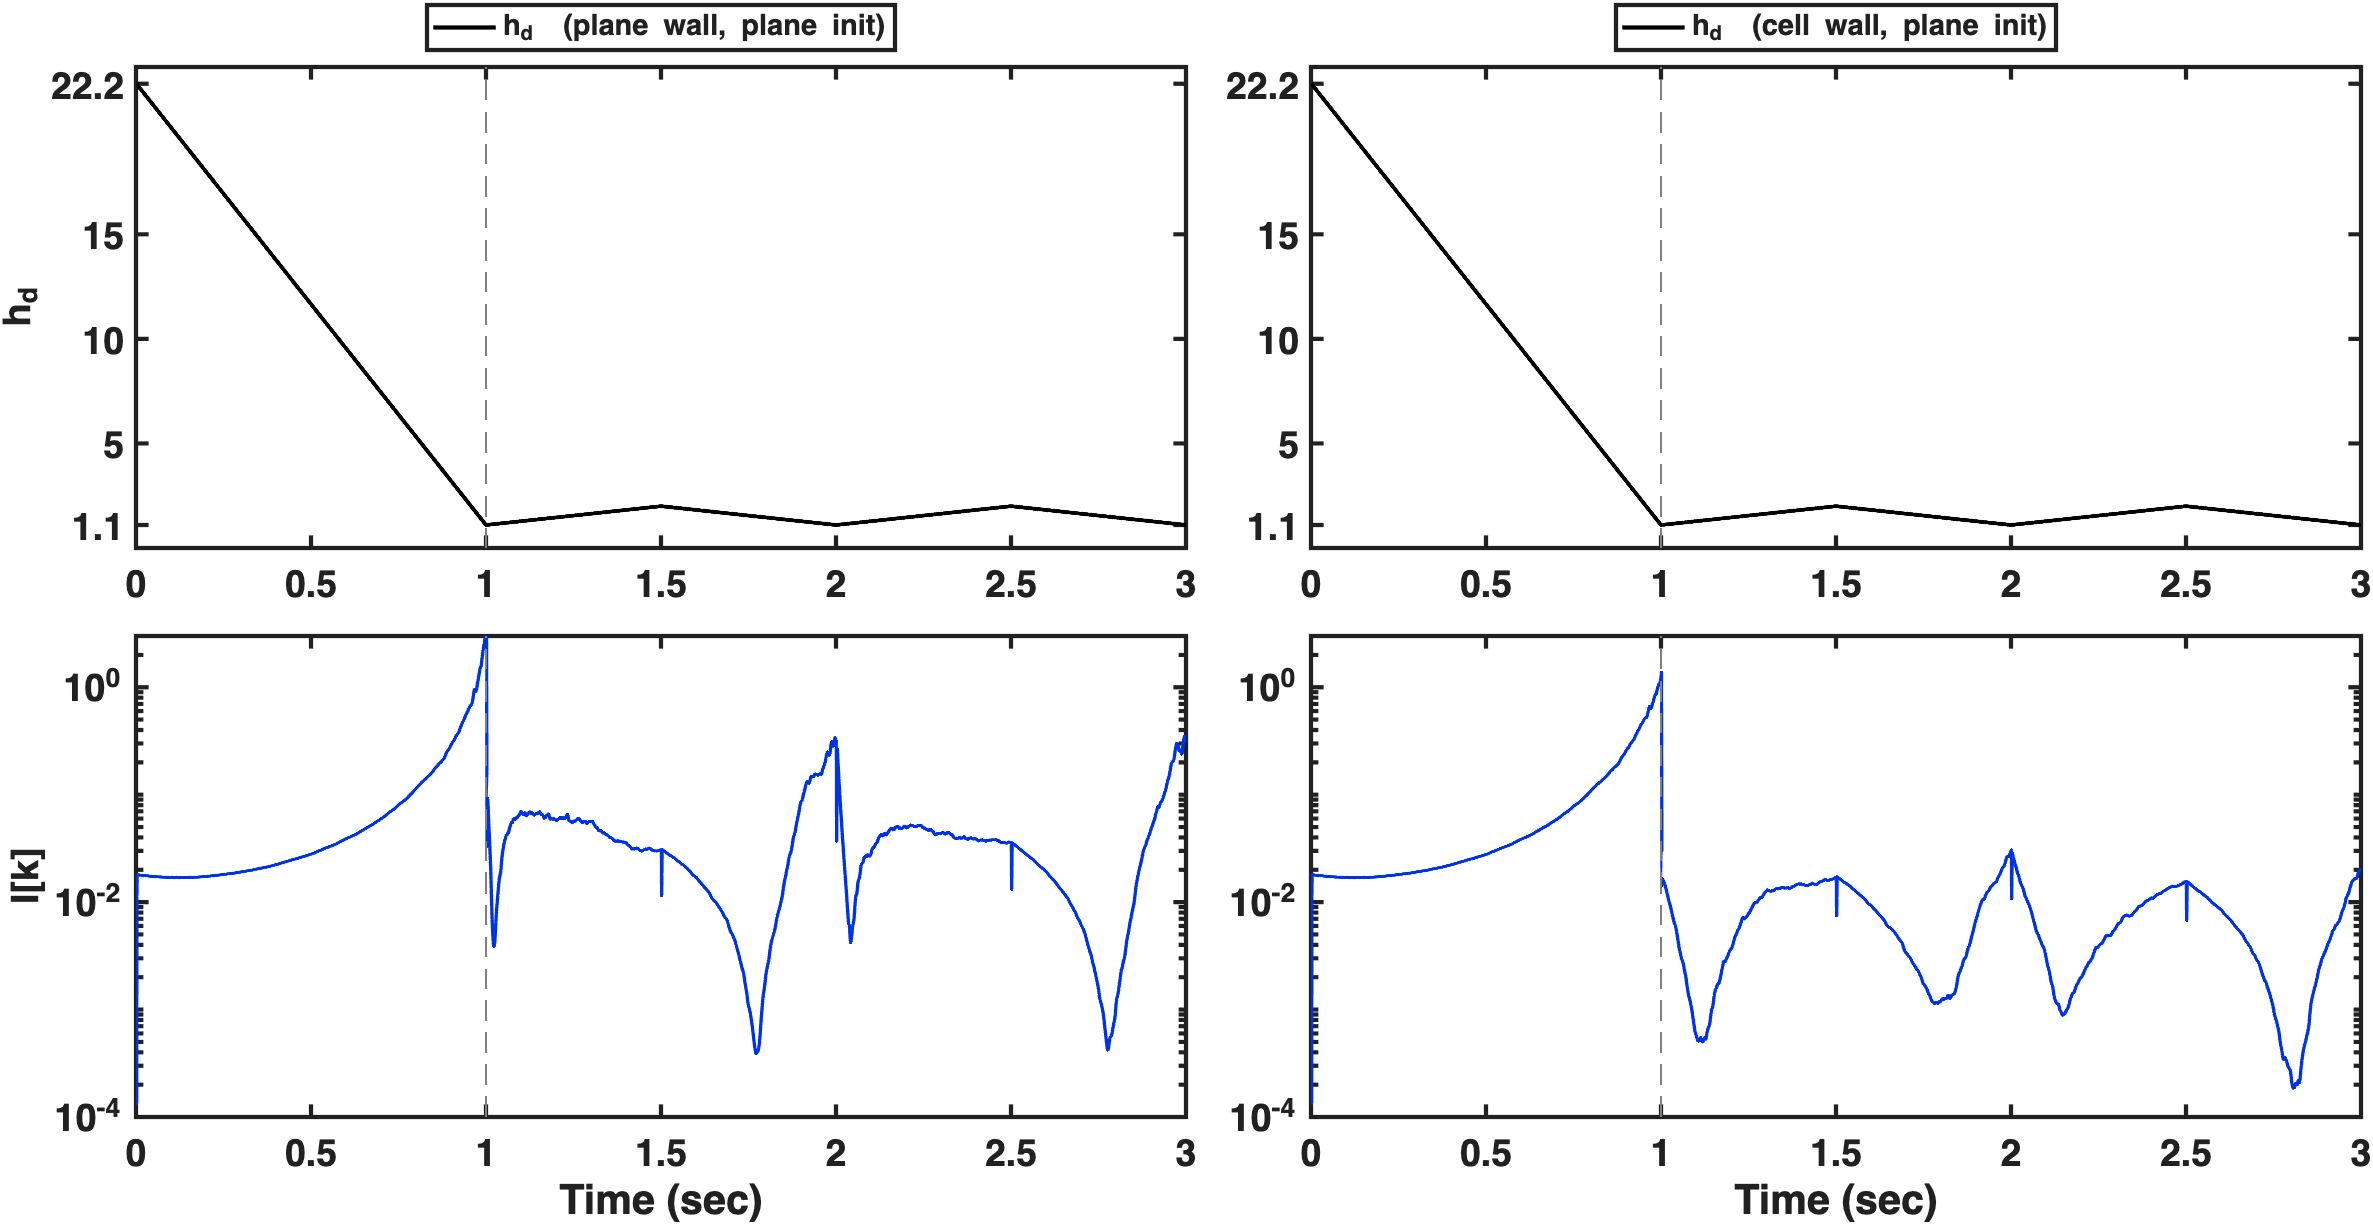
\includegraphics[width=\textwidth]{fig_conly_I_rtri.png}
\end{center}

\end{document}
